\section{Nouveauté}
	
	L'analyse détaillée d'ADtool nous a permis de préciser les fonctionnalités d'analyse qui font défaut à ADTool. Plutôt qu'implémenter ses fonctionnalités directement dans ADTool et ainsi risquer de surcharger ce logiciel nous avons décidé de créer un nouveau logiciel nommé Glasir qui utilise ADTool comme éditeur d'arbre. Nous avons ainsi AdTool qui se charge de la partie \textit{édition des arbres} et notre logiciel qui se charge de la partie \textit{analyse}. Nous avons choisi d'implémenter trois fonctionnalités qui à nos yeux répondent le mieux au besoin d'un expert en sécurité.

	\subsection{Optimiseur}
		% Justifier utilité
		% Présentation fonctionnalité
		% Parler algo
		% Exemple
		
		Actuellement, une fois que l'expert a obtenu son arbre complet (qui peut se composer de plusieurs milliers de noeuds), il ne peut pas facilement identifier le chemin le moins couteux (selon un paramètre donné).
		Il s'agit en effet d'un travail manuel, relativement fastidieux, qui doit être recommencé à chaque modification de l'arbre.
		
		Pourtant, il s'agit d'une méthode systématique, qui peut être implémentée dans notre logiciel.
		Pouvoir identifier automatiquement le chemin optimal ferait ainsi gagner beaucoup de temps à l'expert.
		
		L'optimiseur prendrait donc en entrée:
		\begin{itemize}
			\item un arbre provenant du projet ;
			\item le paramètre à prendre en compte ;
			\item le critère ($min$ ou $max$).
		\end{itemize}
		
		Nous optiendrons en sortie un nouvel arbre (qui sera un sous ensemble de l'arbre d'entrée), contenant le chemin optimal. 
		L'utilisateur pourra ensuite le traiter comme un tout nouvel arbre, en fonction de son besoin.
		
		Nous allons maintenant détailler l'algorithme utilisé. Il s'agira d'une fontion récursive.

		\begin{lstlisting}
opti(racine, param, crit):
	l_fils = fils(racine)

	if vide(l_fils):
		return

	if mode(racine) == ou:
		v = param(l_fils[0])

		for n in l_fils[1:]:
			v = crit(v, param(n))

		for n in l_fils:
			if not defense(n) and param(n) != v:
				delete(n) // will delete subtrees as well
	
	for n in fils(racine):
		opti(n, param, crit)
		\end{lstlisting}

		L'algorithme modifiera l'arbre en l'état (c'est pour cela que nous le ferons travailler sur une copie de l'arbre).
		\begin{itemize}
			\item \verb|racine| correspond au noeud à partir duquel nous élaguerons l'arbre.
			\item \verb|param| est une fonction renvoyant une valeur pour un noeud donné.
			\item \verb|crit| est une fonction prenant en paramètre deux valeurs et renvoie la valeur à \og garder \fg.
			\item \verb|fils| est une fonction renvoyant une liste de noeuds, correspondants aux fils du noeud passé en paramètre.
		\end{itemize}
		Ainsi, pour lancer l'optimisation, nous appelerons \verb|opti| avec la racine de l'arbre en paramètre.

		Prenons en exemple l'arbre exemple en annexe.
		Si on veut trouver le chemin optimal, avec en paramètre le coût, et en critère la fonction $min$, on obtiendra l'arbre de la figure \ref{fig:arbre_post_opti}.

		\begin{figure}
			\centering
			\includegraphics[width=0.5\textwidth]{figure/post_optimiseur.pdf}
			\caption{L'attaque idéale est ainsi facilement lisible.}
			\label{fig:arbre_post_opti}
		\end{figure}


	\subsection{Filtre}

		A l'heure actuelle, l'analyse d'arbre de grandes tailles à l'aide d'ADTool est difficile. 
		En effet, ADTool a été pensé prioritairement pour la modélisation des systèmes sous forme d'ADTrees, et moins pour leurs analyses. 
		ADTool met à disposition de l'expert, comme cela a été précisé précédemment, un certain nombre d'outils pour l'assister dans la modélisation de son système, parmi lesquels se trouve la valuation multiple des noeuds de l'arbre. 
		Une des limites d'ADTool est que une fois le système à protéger complétement représenté sous la forme d'un ADTree, l'arbre peut être trop grand pour que l'expert puisse en retirer une information pertinante. Ceci car la recherche doit se faire à la main et devient donc très longue lorsque l'arbre grandit. 

		Dans un certain nombre de cas, l'expert va chercher à se défendre contre un attaquant précis. Dans ces cas, l'expert va chercher à identifier les ressources dont l'attaquant dispose (temps, argent, personnel humain, etc), ce qui peut amener l'expert à ne vouloir conserver que les chemins de l'arbre empruntables par 				l'attaquant en accord ses ressources. Dans ce cas, nous comparerons les ressources de l'attaquant avec les valuations de l'arbre.

		En l'état, ADTool ne permet pas de faire cette sélection. Nous allons donc implémenter cette fonction dans notre logiciel, sous le nom de \textit{filtre}.

		La fonction de filtrage prendra en entrée : 
		\begin{itemize}
		\item L'arbre à filtrer ;
		\item Les valuations de l'arbre servant de critères pour le filtrage ;
		\item Les intervalles de sélection sur les différentes valuations.
		\end{itemize}

		Le filtre proposera deux types d'intervalles à l'expert pour chacune des valuations :
		L'intervalle global, qui devra être respecté par chacun des chemins conservés, dans le sens où la valuation du chemin dans son ensemble rentre dans l'intervalle.
		L'intervalle unitaire, qui devra être respecté par la valuation de chacun des noeuds pour les chemins retenus.

		Il est possible de filtrer l'arbre avec plusieurs paramètres simultanement.
		
		L'arbre retourné par la fonction de filtrage sera l'arbre d'origine élagé. Seuls seront conservés les chemins respectant les intervalles de filtrage.
		
		L'algorithme du filtre sera selon ce modèle :

		\begin{lstlisting}

filtre(racine, rules) :
	for r in rules :
		if not r(racine) :
			delete (racine AND subtree)
			return

	for n in fils(racine) :
		filtre(n, rules)

\end{lstlisting}
	
		Le principe de l'algorithme est récursif.
		Le nombre d'appel récursif sera, au pire, linéaire avec le nombre de noeud de l'arbre.
		La complexité algorthmique est donc correcte.

		Un exemple d'interface pour le filtre est présenté ici :

		\begin{figure}[h!]
			\begin{center}
				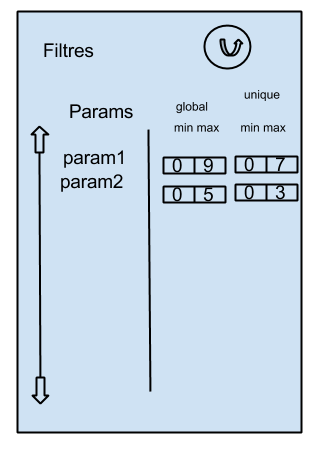
\includegraphics[width=0.35\textwidth]{figure/filtre.png}
			\end{center}
			\caption{Filtre}
			\label{fig:filtre}
		\end{figure}

\subsection{Paramètres de synthèse}

\subsubsection{Les paramètres de base d'ADTool}

ADTool dispose à l'heure actuelle de treize paramètres de base (appelés \textit{domains}), que nous allons présenter succinctement ci-dessous. Nous avons repris les noms (en anglais) qui apparaissent dans le logiciel. 
		
\begin{table*}[!h]
	\centering
	\begin{tabular}{|p{6cm}|p{5cm}|}
  \hline
  \textbf{Paramètre} & \textbf{Valeurs possibles} \\
  \hline
  Difficulty for the proponent (L,M,H) & 
 Low (bas), Medium (moyen), High (élevé) ou l'infini.
\\ \hline
Difficulty for the proponent (L,M,H,E) & 
Low (bas), Medium (moyen), High (élevé), Extreme (extrême) ou l'infini.
\\ \hline
Minimal cost for the proponent (not reusable) & 
Valeurs réelles positives, ou l'infini.\\ \hline
  Minimal skill level needed for the proponent
  & Valeurs entières positives, ou l'infini.\\ \hline
  Minimal time for the proponent (in parallel)
  & Valeurs réelles positives, ou l'infini.\\ \hline
  Minimal time for the proponent (sequential) (\textit{temps minimal séquentiel})
  & Valeurs réelles positives, ou l'infini.\\ \hline
  Overall maximal power consumption & 
  Valeurs réelles positives, ou l'infini.\\ \hline
  Probability of success &
  Valeurs réelles entre 0 et 1.\\ \hline
  Reachability of the proponent's goal in less than k units (in parallel)
  & Valeurs entières de 0 à k. \\ \hline
  Reachability of the proponent's goal in less than k units (sequential)
  & Valeurs entières de 0 à k. \\ \hline
  Satisfiability for the opponent
  & Vrai ou faux. \\ \hline
  Satisfiability for the proponent
  & Vrai ou faux. \\ \hline
  Satisfiability of the scenario
  & Vrai ou faux. \\
  \hline
\end{tabular}
	\caption{Description des paramètres}
	\label{tab:DescriptionParam}
\end{table*}

On voit dans le tableau que des termes particuliers sont utilisés pour désigner les deux parties de l'attaque : l'attaquant et le défenseur. En effet, ADTool permet de se mettre à la place de l'un ou de l'autre. Ainsi, le terme \textit{proponent} désigne l'attaquant (respectivement le défenseur) si on désire son point de vue. L'adversaire (\textit{opponent}) est alors le défenseur (respectivement l'attaquant). % un peu confus. je vois plus un truc du genre : les termes ooponnet et machine designent...

\subsubsection{L'éditeur de paramètres}

L'utilisateur est actuellement cantonné aux valuations présentées ci-dessus, et ne peut pas en créer d'autres sans passer par le code d'ADTool.Celui-ci étant libre de droits, c'est réalisable mais compliqué, surtout que l'utilisateur n'est pas forcément expérimenté en informatique. % Confus et inutile, juste préciser que l'utilisateur ne peut pas avoir de nouveau paramètres.
Nous souhaitons donc faciliter la création de nouveaux paramètres à partir de ceux déjà disponibles et des fonctions mathématiques de base (division, multiplication, min, max, etc). Ces nouvelles valuations pourront ensuite être appliquées aux arbres voulus, de la même manière que pour les paramètres de base. Elles pourront ainsi être utilisées pour analyser les arbres selon de nouveaux critères, et si besoin pour les élaguer à l'aide du filtre que nous allons implémenter.\\

Cette nouvelle fonctionnalité, appelée éditeur de paramètres, prendrait donc en entrée les éléments suivants :
\begin{itemize}[label=\ding{170},font=\color{magenta},parsep=0cm,itemsep=0cm, leftmargin=0cm]
\item un arbre provenant du projet ;
\item les paramètres intervenant dans la synthèse ;
\item les opérations mathématiques appliquées ;
\item le nom du paramètre de synthèse généré.
\end{itemize}

% exemples
		

